\documentclass{article}

%%%%%%%% SKYEPAPHORA %%%%%%%%
\usepackage[margin=1in]{geometry} 
\usepackage{amsmath,amsthm,amssymb,amsfonts}
\usepackage{xcolor}
\usepackage{cancel}
\usepackage[framemethod=tikz]{mdframed}
\usepackage{mathtools}
\usepackage{bm}
\usepackage[font=small]{caption}
\usepackage{graphicx}
\usepackage{enumerate}
\usepackage{setspace}
\usepackage{listings}
\usepackage{multicol}
\usepackage{textcomp}
\usepackage{centernot}
\usepackage{bbm}
\usepackage{mathrsfs}
\usepackage{hyperref}
\hypersetup{
    colorlinks=false,
    linkcolor=blue
    }

\setlength{\fboxsep}{5pt}
% \setlength{\parindent}{0pt}

\newcommand{\define}{\ensuremath \stackrel{\text{def}}{=}}
\newcommand{\Var}{\ensuremath \text{Var}}
\newcommand{\Cov}{\ensuremath \text{Cov}}
\newcommand{\E}{\ensuremath \text{E}}
\newcommand{\myrule}{\rule{\linewidth}{0.5pt}}

\definecolor{gold}{HTML}{A05000}
\definecolor{redd}{HTML}{C00000}
\definecolor{bluu}{HTML}{0000C0}
\definecolor{gren}{HTML}{00B000}

\definecolor{salt}{HTML}{FBFAF9}
\definecolor{pepper}{HTML}{251F18}

\begin{document}
\pagecolor{salt}\color{pepper}

% --- Curvy BCMTFSE ---------
\section{Further Modifications to the BCMTFSE}
One disadvantage of the BCMTFSE is that the extrapolation taking place at either time-endpoint of the MTFSE is \textit{linear.} This disregards what curvature (with respect to time) might be present in the true Time Frequency Spectrum (TFS) within those time-boundary regions. Moreover, this extrapolation is entirely dependent on the time derivative of the MTFSE at those solitary endpoints. For any column of the MTFSE, a lack of smoothness adjacent to these endpoints may result in wildly steep or shallow extrapolations $-$ perhaps of the wrong signature $-$ all due to a ``bump in the road," so to speak.

FIGURE

\section{Boundary Correction for the MTFSE using Second-Order Taylor Approximations}
One way to account for possible time-boundary curvature is to extend the estimate into these regions by way of \textit{second} order Taylor approximations. This approach is not without its disadvantages. In fact, by incorporating the MTFSE's second time derivative into the mix, we obtain an estimate \textit{less smooth} than the original BCMTFSE. An opportunity to apply non-linear extrapolations in this context is, nevertheless, worth investigating.

\subsection{Constructing the CBCMTFSE}
Recall that, according to Non-Stationary Quadratic Inverse Theory, the TFS of a non-stationary process may be approximated by (??), with accompanying eigenvalue equation (??). Recall, further, that this may be applied when the TFS is restricted to a time region, or \textit{block}, indexed by $b$. The eigenvalue equation becomes:
\begin{flalign}
        S_b(t,f) &\approx \sum_{l=0}^{L_b} a_{l,b}(f)A_l(t-b). 
    \intertext{We now consider an approximation formed by the first 3 terms of $S_b(t,f)$'s Taylor expansion (rather than the first 2, as per the technique from section (??)).}
        S_b(t,f) \approx  S_b(t_b,f) 
                &+ S^{(1)}(t_b,f)(t-t_b) + \frac{1}{2}S^{(2)}(t_b,f)^2
\end{flalign}
Similarly to section (??), we set these approximations equal to one another, multiply each side by $A_m(t-t_b)$ for some arbitrary $m\in \{0,\dots,L_b\}$, and then sum over time in-block. Since $A_m(t-t_b)$ is independent of $l,$ and $a_{l,b}(f)$ is independent of time, the order of the sums can be switched to obtain
\begin{flalign}
        &\;\;\sum_{l=0}^{L_b} a_{l,b}(f) \sum_{t=b}^{b+B-1}A_m(t-b)A_l(t-b) \notag
        \\[5pt]
        \approx 
        &\sum_{t=b}^{b+B-1} A_m(t-b)\Big[ S_b(t_b,f) +
            S^{(1)}(t_b,f)(t-t_b) + 
            \frac{1}{2}S^{(2)}(t_b,f)^2\Big] 
\end{flalign}
The $A_l$ sequences are orthogonal such that
\begin{equation}
    \sum_{t=0}^{B-1}A_i(t)A_j(t) = B\;{\large\mathbbm{1}}\{i=j\}.
\end{equation}
Thus, equation (??) may be simplified to only include its non-zero terms, each of whom require $m=l$. 

We now wish to formulate a system of approximations from equation (??) at orders $l= 0,1,2$; a set of expressions rather too wide to fit on the page whilst also complying with this document's formatting expectations.

For ease of notation, then, we let $T_b$ denote the set $\{b,b+1,\dots,b+B-1\},$ that is, the range of times which define block $b.$ Furthermore, we define the following function,
\begin{flalign}
    \omega_p(l,b) &\define \sum_{t\in T_b}A_l(t-b)(t-t_b)^p.
\end{flalign} 
The following are true for $l= 0,1,2$: 

\small\begin{flalign}
    B\, a_{0,b}(f) 
        &\approx S_b(t_b,f)\omega_0(0,b) +
        \boxed{S_b^{(1)}(t_b,f)\omega_1(0,b)} + 
        \frac{S_b^{(2)}(t_b,f)}{2}\omega_2(0,b)
        \\[8pt]
    B\, a_{1,b}(f) 
        &\approx \boxed{S_b(t_b,f)\omega_0(1,b)} +
        S_b^{(1)}(t_b,f)\omega_1(1,b) + 
        \boxed{\frac{S_b^{(2)}(t_b,f)}{2}\omega_2(1,b)}
        \\[8pt]
    B\, a_{2,b}(f) 
        &\approx S_b(t_b,f)\omega_0(2,b) +
        \boxed{S_b^{(1)}(t_b,f)\omega_1(2,b)} + 
        \frac{S_b^{(2)}(t_b,f)}{2}\omega_2(2,b)
        \\[-5pt] \notag
\end{flalign}

Noting that $A_1(t-b)$ and $A_1(t-b)(t-t_b)^2$ are even functions of time, and that $A_0(t-b)(t-t_b)$ and $A_2(t-b)(t-t_b)$ are odd in the same respect, the boxed terms in approximations (??) through (??) are each valued at zero. Hence,
\begin{flalign}
    B\, a_{0,b}(f)
        &= S_b(t_b,f)\omega_0(0,b) + \frac{S_b^{(2)}(t_b,f)}{2}\omega_2(0,b)  
        \\[5pt]
    B\, a_{1,b}(f)
        &= S_b^{(1)}(t_b,f)\omega_1(1,b)  
        \\[5pt]
    B\, a_{2,b}(f)
        &= S_b(t_b,f)\omega_0(2,b) + \frac{S_b^{(2)}(t_b,f)}{2}\omega_2(2,b)  
        \\[-5pt] \notag
\end{flalign}

\noindent Solving for $S_b(t_b,f)$ and its first and second order time derivatives, we obtain the estimates
\begin{flalign}
    \hat S_b(t_b,f) 
    &= \frac
        {B\Big(\hat a_{2,b}(f)\omega_2(0,b) -\hat a_{0,b}(f)\omega_2(2,b) \Big)}
        {\omega_0(2,b)\omega_2(0,b) - \omega_0(0,b)\omega_2(2,b)}
    \\[5pt]
    \hat S_b^{(1)}(t_b,f) 
    &= B\,\hat a_{1,b}(f)\omega_1(1,b)^{-1} 
    \\[5pt]
    \hat S_b^{(2)}(t_b,f) 
    &= \frac
        {2B\Big(\hat a_{0,b}(f)\omega_0(2,b) -\hat a_{2,b}(f)\omega_0(0,b) \Big)}
        {\omega_0(2,b)\omega_2(0,b) - \omega_0(0,b)\omega_2(2,b)},
\intertext{ where the expansion coefficients $\hat a_l$ are estimated by}
    \hat a_{l,b}(f) 
    &= \frac{K}{B\alpha_l}
        \sum_{t=b}^{b+B-1}\hat S_{b}^{(SW)}(t,f)A_l(t-b),
\intertext{and where $\hat S_{b}^{(SW)}$ denotes the SWHRS. Alternatively, $S_b$ and can be estimated in terms of its second time-derivative, and vice versa:}
     \hat S_b(t_b,f) 
     &\approx 
     \omega_0(0,b)^{-1}
     \left(B\, \hat a_{0,b}(f) - \frac{S_b^{(2)}(t_b,f)}{2}\omega_2(0,b)\right)
     \\
     \hat S_b^{(2)}(t_b,f)
     &\approx 
     2\omega_2(2,b)^{-1}
     \left(B\, \hat a_{2,b}(f) - S_b(t_b,f)\omega_0(2,b)\right),
\end{flalign}
which is convenient from the perspective of one who wishes to implement this chapter's techniques via code. 

The proposed TFS estimator for timepoints in \textit{non-}boundary regions is simply $\hat S_b(t_b,f)$ per equation (??). In time boundary regions, however, we extend the estimate as follows.
\begin{equation}
    \hat S_b (t_b+h,f) \stackrel{def}= 
    \hat S_b(t_b) + h\hat S^{(1)}_b(t_b) + \frac{h^2}2 \hat S^{(2)}_b(t_b)
\end{equation}
That is to say, similarly to the BCMTFSE, $\hat S_b (t,f)$ is a \textit{combined} estimator defined piecewise as a function of blockwidth. Due to the inherent curvature of these extensions into time boundary regions (in combination with the lack of smoothness which comes from including second order information in the Taylor expansions leading up to this point), we dub this estimator the \textit{Curvy Boundary Corrected Modified Time Frequency Spectrum Estimator,} or CBCMTFSE.\footnote{Okay, okay, \textit{tentatively.}} 
For ease of abbreviation, the terms BCMTFSE and CBCMTFSE will be respectively truncated to BC and CBC for the remainder of the document.   

%%%                                                                                    %%%
%%% ------------ SKYE YOU CAN START HERE IF YOU WANT TO WORK ON CHAPTER 3 ------------ %%%
%%%                                                                                    %%%

% CODE: this is easy stuff, do the cbcmtfse and get some momentum going. Pretty pictures if you feel bad about yourself
% Finish up section 3.1, see if you can get to a formal conclusion.

\subsection{Performance of the CBCMTFSE using simulations}

It's not immediately obvious whether our new estimator should perform any better than the BC. As discussed, it \textit{may} be advantageous to assume the true TFS has some quadratic structure within time boundary regions, as we won't often expect a sudden linear trend on either side of the MTFSE for a non-stationary time series. However, the CBC does not perform these extrapolations from the \textit{same} MTFSE as the BC. 

Let me explain: the estimator $\hat S_{X,b,M}(t_b,f)$ from equation (?? - chapter 2) is quite different from the estimator $\hat S_b(t_b,f)$ in equation (??). In other words, the time-\textit{center} regions of the BC and CBC are different from one another; the extrapolation is not all that distinguishes the two estimators. The extra information incorporated into the CBC's time-center region may affect the smoothness, bias, and variance properties enjoyed by the BC's time-center, \textit{on top} of whatever discrepancies occur in the time-boundary regions.

Thus, the following sections compare how the BC and CBC behave given simulated data. We will construct 3 examples, covering a few different types of time series: stationary white noise, stationary AR(2), and non-stationary UMP. For each example, we will produce $M=100$ realizations. Figures will display the mean values over all $M$ simulations, along with the $2.5^{th}$, $50^{th}$, and $97.5^{th}$ quantiles. The spectrograms themselves will be featured, in addition to rows/columns at some randomly selected common time-point and frequency. 

\subsubsection{Example A: Stationary Processes}

Before examining processes which actually \textit{evolve} over time, let us play with some trivial examples. As we construct the following time series, assume $N=1000$ and $\Delta t = 1$, giving us a Nyquist frequency of $1/2$. The frequency domain will be discretized to $N_f = 2^{\lceil\log_2(N)\rceil}+1 = 1025$ frequencies on the interval $[0,1/2]$. 
\begin{flalign}
     z(t) &\sim w\big(0,\;\sigma_z^2 = 10^2\big)      \\
     y(t) &= 0.5\,y(t-1) - 0.5\,y(t-2) + \epsilon(t)  \\
     \epsilon(t) &\sim w\big(0,\;\sigma_\epsilon^2 = 10^2\big)
\end{flalign}
We will examine the CBC for both $z$ and $y$. This gives some anecdotal insight into the estimator's performance for pure white noise, $z$, in addition to an example of a stationary AR(2) process, $y$. Note that $z$ and $\epsilon$ are identically distributed, but are distinct realizations. 

The theoretical spectrum $S_X(f)$ of $z(t)$ should be obvious: uniformly distributed power at $\sigma_z^2$ on the frequency interval $[0,1/2]$. The corresponding TFS matrix will have mutually identical rows \textit{and} identical columns, since its power does not change with respect to time \textit{nor} frequency. Its graphical depiction, via heat map, is just a rectangle of one solid colour. 

The series $y(t)$ is AR(2) and stationary, thus its theoretical spectrum is known to be
\begin{equation}
    S_Y(f) = \frac{\sigma_\epsilon^2}{\Big|1 - 0.5e^{-i2\pi f} + 0.5e^{-i4\pi f}\Big|^2}. \qquad
\end{equation}
Stationarity dictates that $S_y(f)$ is independent of time, implying the corresponding TFS matrix will have mutually identical rows. A heat map of the true TFS will therefore display vertical lines of colour as they vary across an independent frequency axis. 

Figure (??) displays heat maps for the theoretical TFS matrices $S_X(t,f)$ and $S_Y(t,f)$, followed by heat maps of the BC and CBC as computed by R. For both series, the BC is apparently prone to underestimation, and this bias is improved in both cases by the CBC. However, the CBC is less smooth than the BC, and the bottom left plot demonstrates how the CBC's quadratic extrapolation may have backfired in the first time boundary region of $z(t)$ due to overestimation.

Overall, we observe that the CBC performs slightly better than the BC does in the stationary case. Implications of these results will be discussed later in the chapter.

% \footnote{We can think of both series as UMPs if we consider $c(t) = 1$ to be their common modulating function for $t \in \{0,\dots,N-1\}$. We'll use this to plot their theoretical spectrograms for the purpose of comparing them to our estimates, later on.}

% Under more general conditions than the stationarity we've constructed, the MTFSE and its boundary corrected counterparts have been compared to established TFS estimators: the HRS and SWHRS [??]. We will add another link to this chain of comparisons by simply comparing the CBC to the BC, both of whom include extrapolations into the time boundary regions. Caring about these extrapolations is counter-intuitive in the stationary case, of course, where we expect the spectra not to evolve over time - however, a good estimator should be still able to detect a \textit{lack} of evolution in this sense.

\begin{figure}
    \centering
    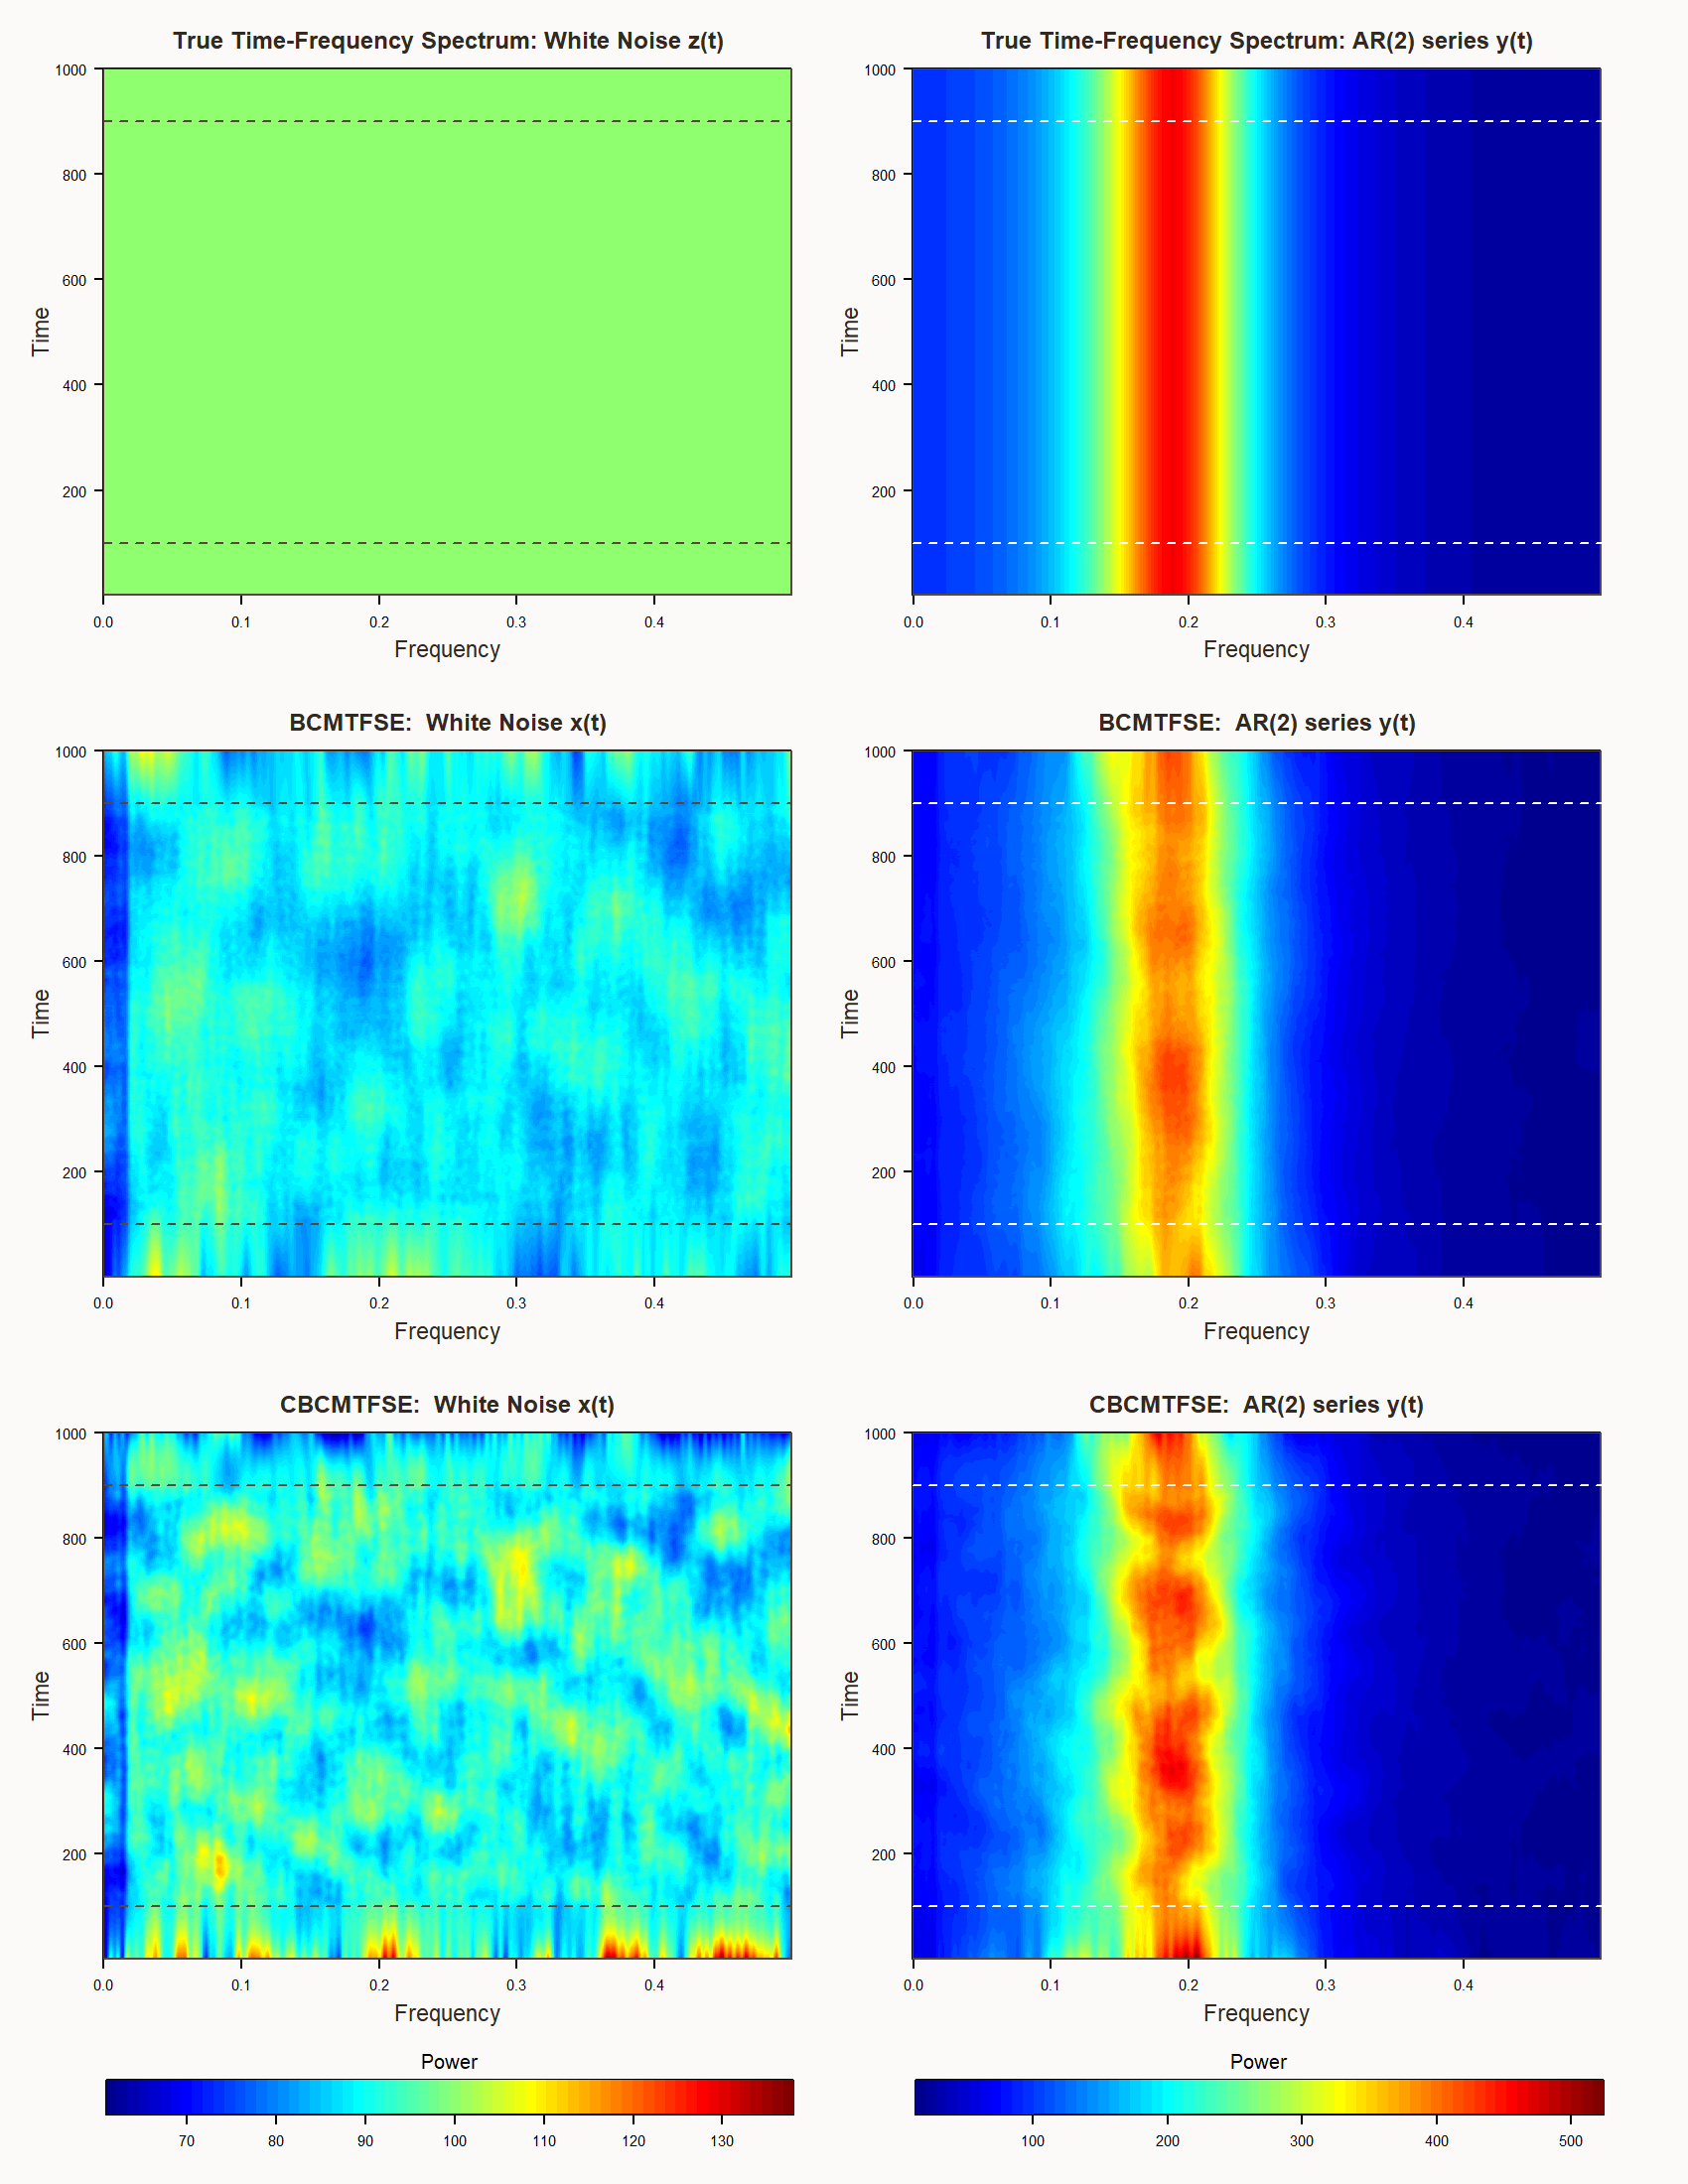
\includegraphics[width=\linewidth]{Fig/sgrams_Noise-AR2_B200_letterbox.png}
    \caption{Performance of BC and CBC spectrograms as compared to the true TFS matrices of series $z(t)$ and $y(t)$. The results featured are the mean values taken across $M=100$ simulations with a common blockwidth of $B=200$. The black, dotted, horizontal lines indicate the threshold for the time boundary regions corresponding to this blockwidth.}
    \label{fig:1}
\end{figure}

\subsubsection{Example B: Uniformly Modulated Process 1}
In the previous section, aside from white noise, we considered a stationary AR(2) series. Now, let us examine how these estimators perform when a similar series is uniformly modulated to no longer be stationary. The series we'll use is exactly the one featured in example 1 of [??] $-$ this will provide a graphical sanity check in terms of whether we've authentically reproduced the BC as per its original construction.\footnote{Note that the corresponding spectrograms in [??] are oriented such that the horizontal axis represents time, unlike the spectrograms in figure (??) of this document.}

Suppose we have the following set of time series:
\begin{flalign}
    \epsilon(t) &= w\big(0,\;\sigma_\epsilon^2 = 10^2\big).       \\
    c(t)        &= \exp\left\{\frac{-(t-500)^2}{2(200)^2}\right\} \\
    Y(t)        &= 0.5\,Y(t-1) - 0.5\,Y(t-2) + \epsilon(t)        \\[5pt]
    X(t)        &= c(t)Y(t)
\end{flalign}


As the reader can see, $X(t)$ is UMP, $Y$ is the same stationary AR(2) process featured in the previous section, and $c(t)$ is a modulating function. Recall that since $X(t)$ is uniformly modulated, its TFS matrix at $(t,f)$ is given by
\begin{equation}
    S_X(t,f) = c^2(t)\cdot S_Y(f).
\end{equation}
Figure (??) demonstrates how the BC and CBC perform when trying to estimate $S_X(t,f)$. Similarly to Example A, we see that the CBC improves on the BC's underestimation, but at the cost of the CBC's shape being slightly compromised due to a reduction in smoothness. 

\begin{figure}[h!]
    \centering
    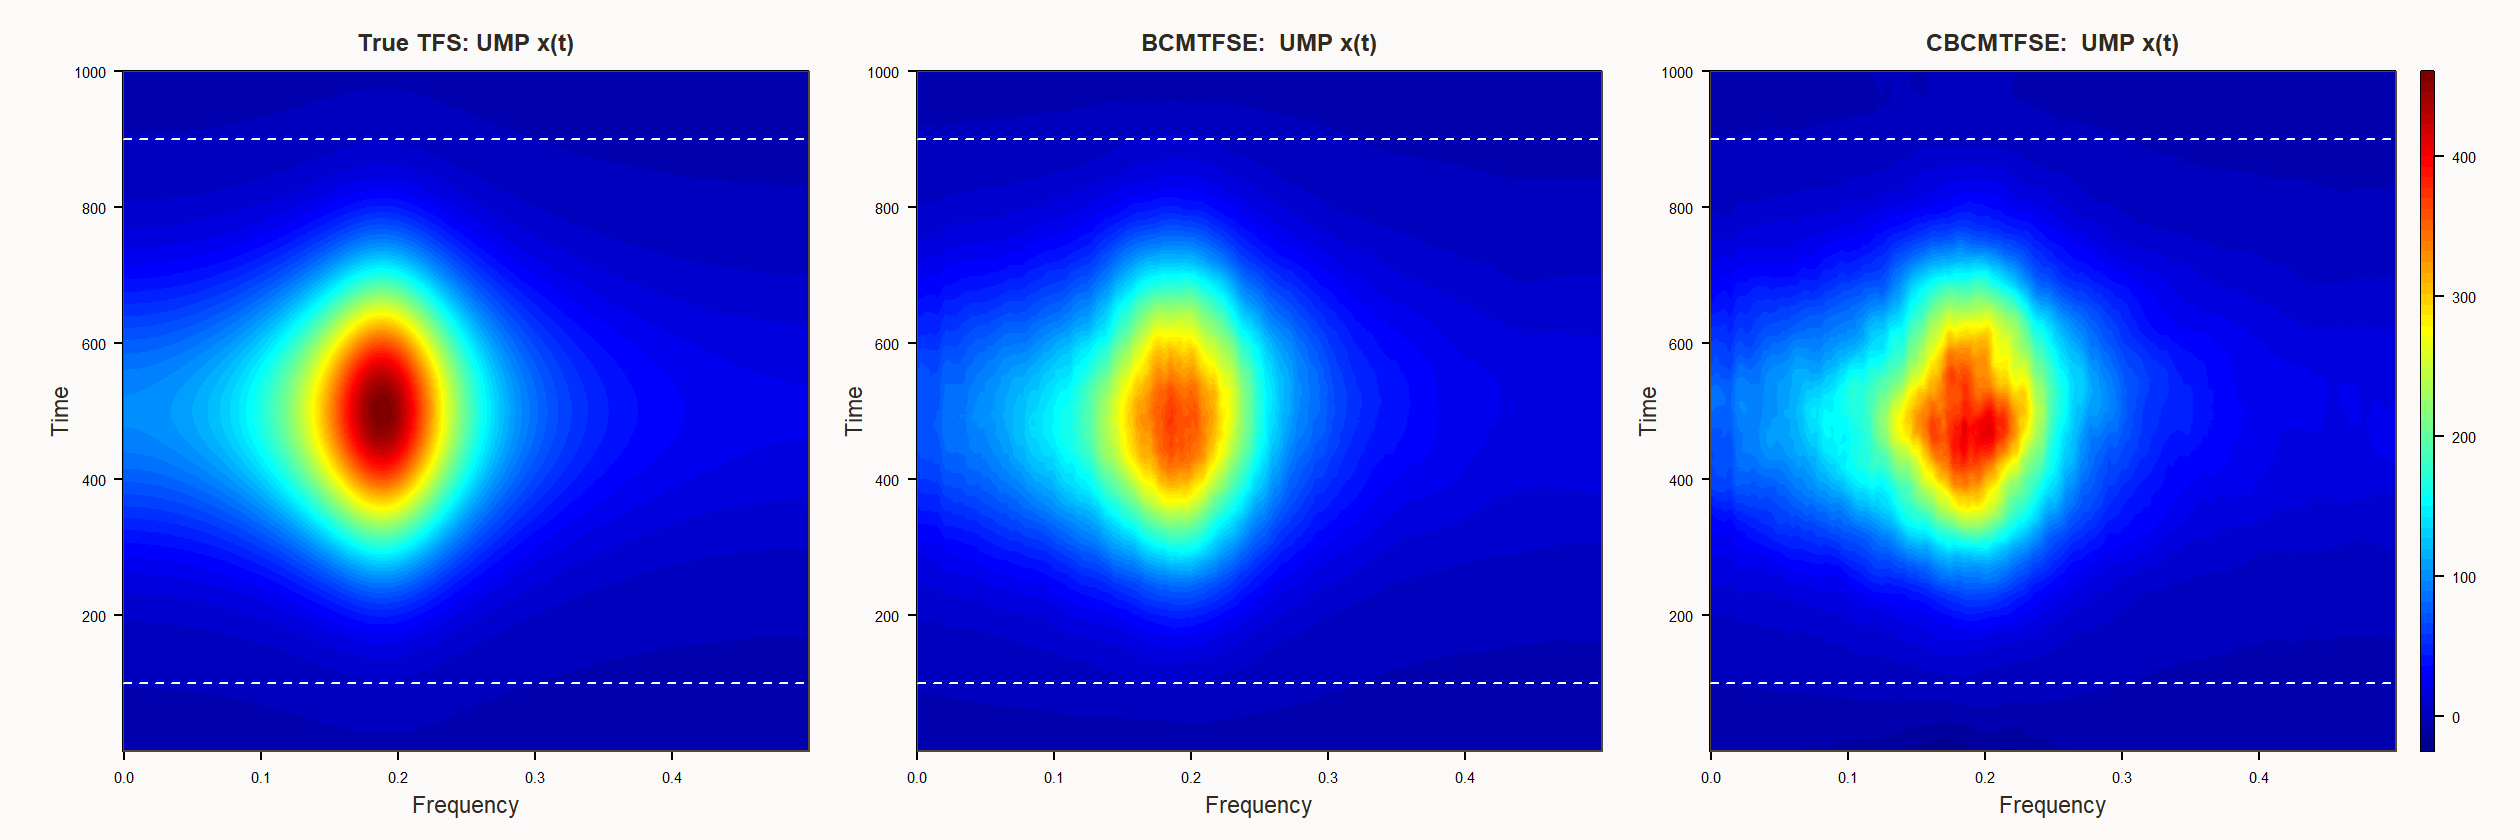
\includegraphics[width=\linewidth]{Fig/sgrams_UMP_B200_letterbox.png}
    \caption{From left to right: the true TFS, BC, and CBC heat maps for the $X(t)$ given in Example B. The results featured are the mean values taken across $M=100$ simulations with a common blockwidth of $B=200$. The white, dotted, horizontal lines indicate the threshold for the time boundary regions corresponding to this blockwidth.}
    \label{fig:enter-label}
\end{figure}

\subsubsection{Example C: Uniformly Modulated Process 2}
The modulating function from the previous example is a bit convenient in that the resulting UMP's evolutionary spectral power was largely concentrated in the time-center region, where we expect the spectrograms to perform most reliably. A lot of what figure (??) emphasizes, therefore, is the discrepancy between what parts of these spectrograms were \textit{not} subject to time-boundary extrapolations.

In contrast, we now adjust the modulating function so that we expect power to be concentrated more heavily towards the time-boundary regions of the UMP's TFS and its estimators. Let $X(t)$ and $Y(t)$ maintain the definitions given in equations (??) and (??), respectively, but take $c(t)$ to now be
\begin{equation*}
    c(t) = 1 - \exp\left\{\frac{-(t-500)^2}{2(200)^2}\right\}.
\end{equation*}.

\begin{figure}
    \centering
    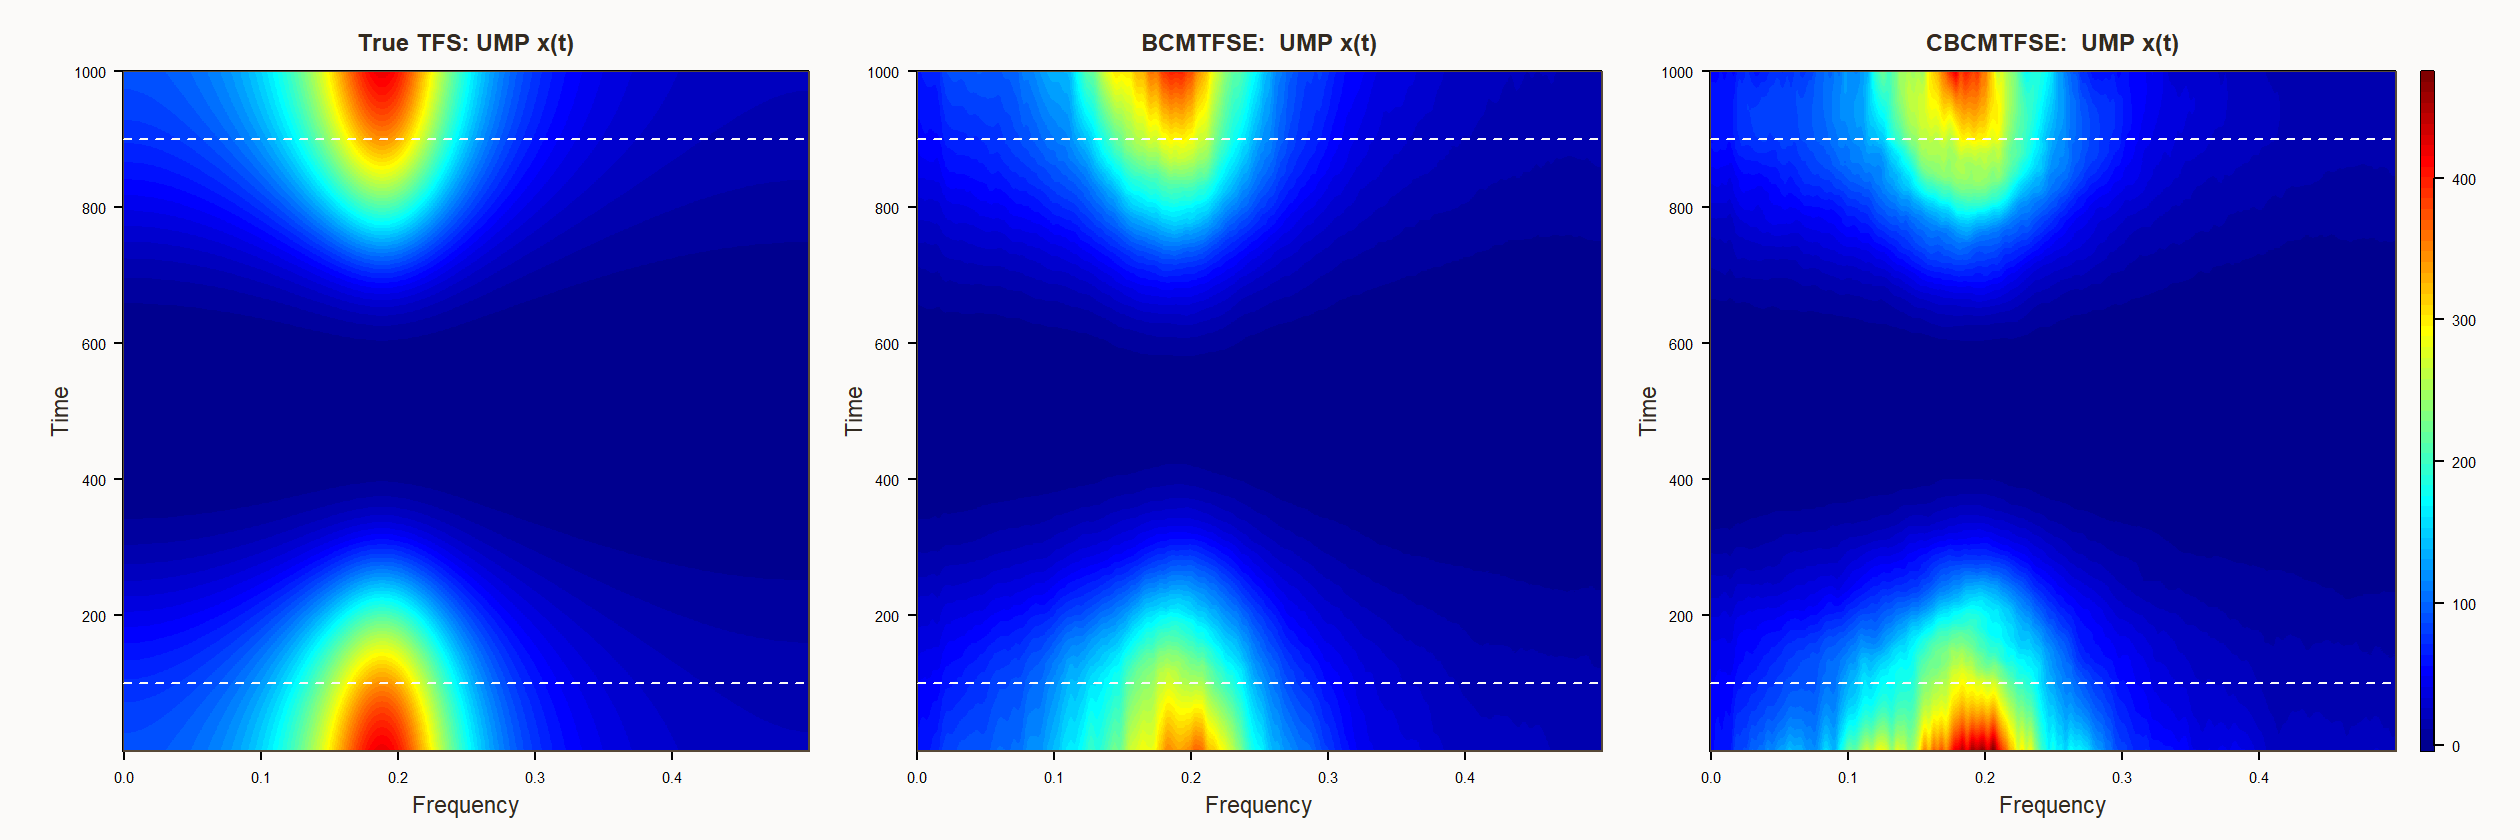
\includegraphics[width = \linewidth]{Fig/sgrams_UMP_B200_rev_letterbox.png}
    \caption{From left to right: the true TFS, BC, and CBC heat maps for the $X(t)$ given in Example B. The results featured are the mean values taken across $M=100$ simulations with a common blockwidth of $B=200$. The horizontal dotted lines indicate the threshold for the time-boundary regions corresponding to this blockwidth.}
    \label{fig:enter-label}
\end{figure}

Figure (??) demonstrates how the BC and CBC perform now that the sites of extrapolation are emphasized. It becomes clear that the CBC is better equipped to estimate the TFS at these regions, which is what we would expect given the curvature of $c(t)$ at such time intervals. 

The width of the time-boundary region is proportional to the chosen blockwidth $B$. To demonstrate how effectively the BC and CBC extrapolate over a greater period of time, particularly in proportion to original series length, we produce Figure (??) using $B=400$. This is in contrast to Figure (??), which used $B=200$. Again, we see that the CBC is slightly less prone to underestimation, most notably in the first (chronological) time-boundary region.

\begin{figure}[h!]
    \centering
    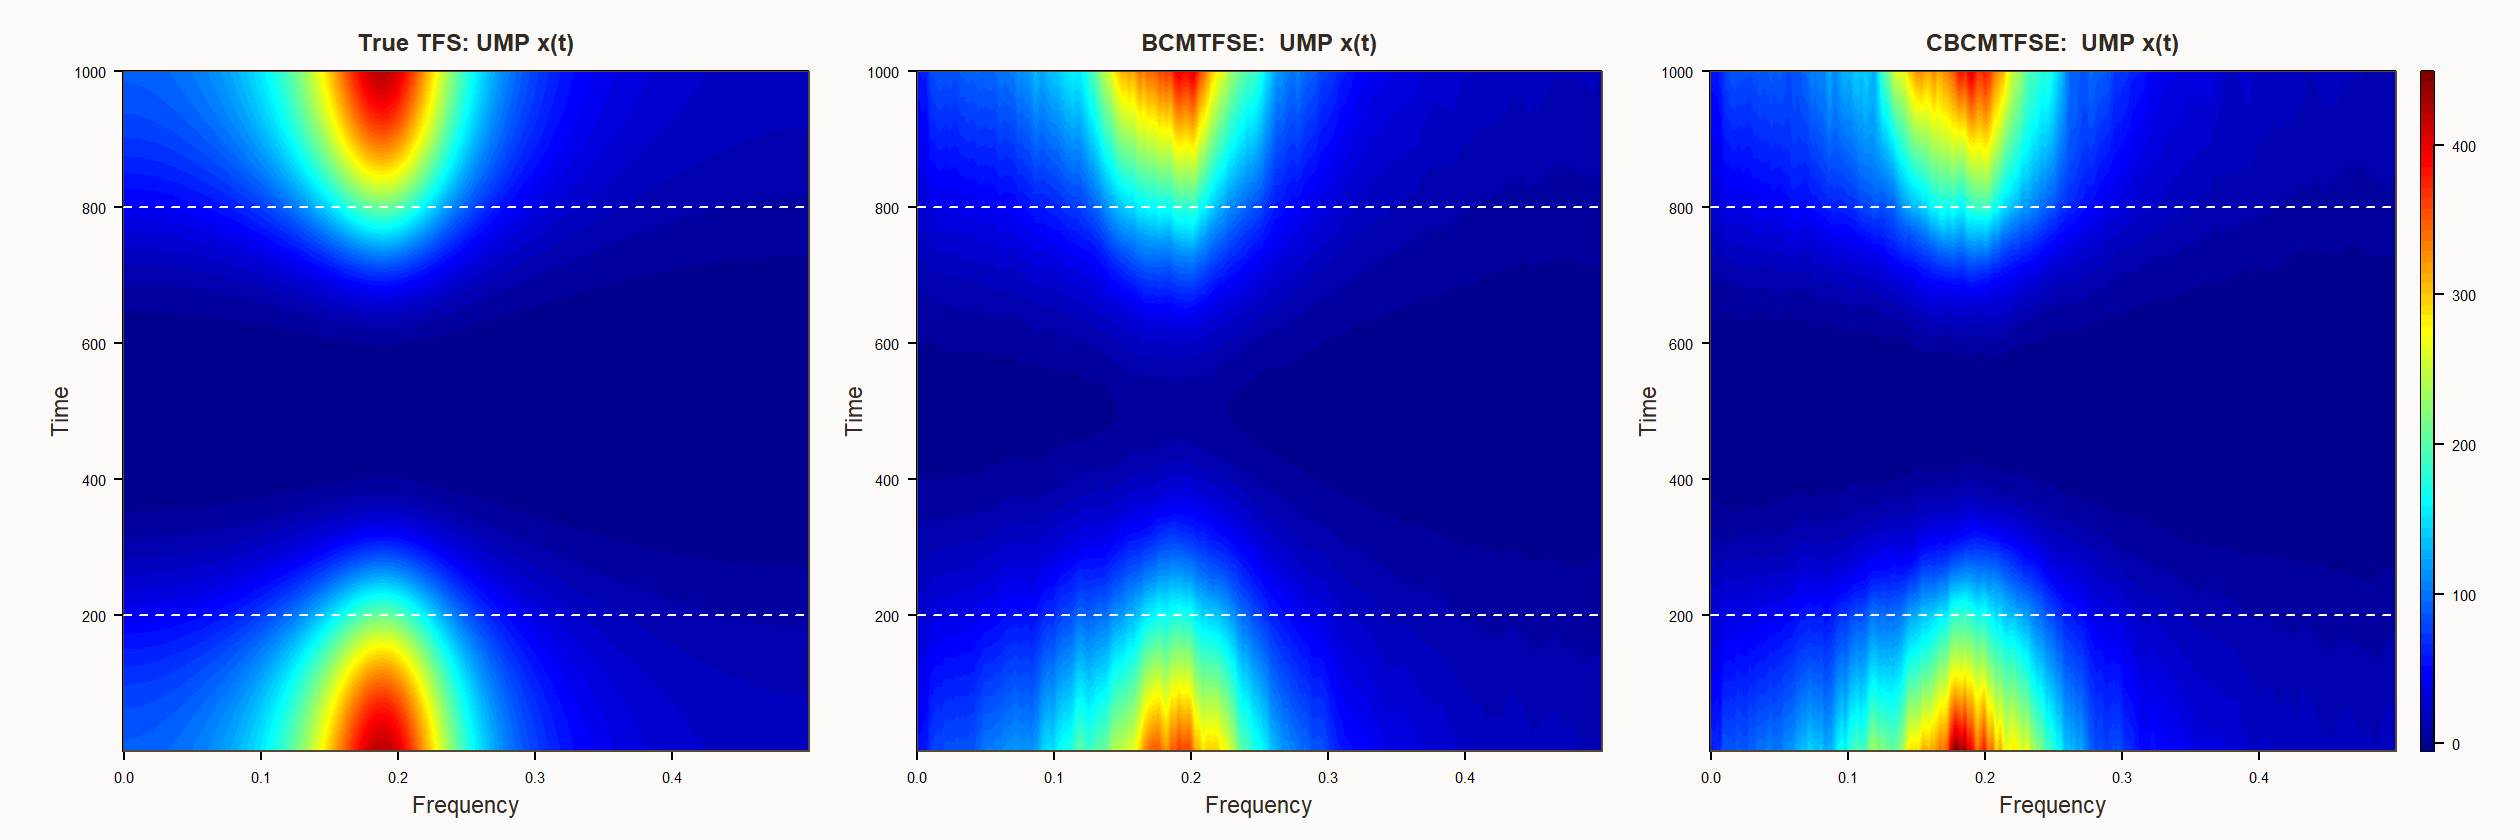
\includegraphics[width = \linewidth]{Fig/sgrams_UMP_B400_rev_letterbox.png}
    \caption{These plots represent the same estimators as those in Figure (??), but based on an increased blockwidth: $B=400$. Thresholds for time-boundary regions are indicated by horizontal dotted lines.}
    \label{fig:enter-label}
\end{figure}

\subsubsection{Example: Non-Stationary, Non-Uniformly Modulated Process}







% --- ESTIMATING C ---------
\section{Estimating Modulating Functions of UMPs}
% Motivation and Review
Consider a UMP's time frequency spectrum, restricted to discrete sets of both time and frequency such that the TFS can be represented by a matrix. Any given row of this matrix represents the frequency spectrum of the UMP at a fixed, corresponding time point. As we move through time, the proportional structure of that frequency spectrum remains intact, with peaks and troughs expanding and contracting in unison. This restriction affords mathematical advantages in that the modulating function responsible for the UMP's non-stationarity is captured in the relative values of the TFS from row to row. Previous work [??] has been done to develop estimates for said modulating function, however, the established techniques are limited in that BLABLABLA. This section examines alternative approaches to estimating the UMP's modulating function.

\subsection{Derivation of Techniques}
Consider the UMP $X(t) = c(t)Y(t).$ Denote its TFS matrix by $\mathbb S_X $, with entries $S_X(t,f)$ for times $t \in T =\{1,\dots,N\},$ and Fourier frequencies $f \in \{f_1, \dots, f_{N_f}\}$. We choose to begin at time $t=1$ rather than $t=0$, so that $t$ corresponds exactly to the $t^{th}$ row of $\mathbb S_X$. Recall that since $X(t)$ is uniformly modulated, its TFS matrix is such that
\begin{flalign}
    S_X(t,f) &= g(t) S_Y(f),
\intertext{or in matrix notation, }
    \mathbb S_X &= \vec g \cdot S_Y,
\intertext{where $g$ is the column vector $g(t) = c^2(t)$, and $S_Y$ is a row vector representing the spectrum of $Y(t)$. Note that $S_Y$ is time-independent thanks to $Y(t)$ necessarily being stationary.}\notag\\[-25pt] 
\intertext{\indent If we take the sum over each row of $S_X$, we're left with a vector $V_X(t)$ representing the total spectral power at each timepoint $t$:}
    V_X(t) &\define \sum_{i=1}^{N_f} S_X(t,f_i) \\
           &= g(t)\sum_{i=1}^{N_f} S_Y(f_i)
\intertext{\indent Since the entire sum $\sum_{i=1}^{N_f} S_Y(f_i)$ is independent of time, it simply acts as a constant. Therefore, the structure of $V_X(t)$ will resemble that of $g(t)$ to some extent: the proportion between any two entries in $V_X(t)$ should reflect the proportions between corresponding entries of $g(t)$. To estimate $c^2(t)$ then, an approach might be to examine each $V_X(t)$ as a proportion of $V_X(1)$, and simply store those proportions as a function of time. In fact, this can be done relative to any $t_0 \in T$:}
d_{t_0}(t) &\define V_X(t)/V_X(t_0).
\end{flalign}
The function $d_1(t)$ (where $t_0=1$ is chosen without loss of generality) is a basic proposed estimate of the UMP's squared modulating function, which we will denote $\hat g$. The caveat, here, is that $\hat g$ can only be constructed up to some normalizing constant. Namely, $d_{1}(t)$ at time $t = 1$ is forced to have unit value. Although the issue of relying on a normalizing constant remains, a general improvement on the estimate $\hat g = d_1$  can be made by incorporating the information from every $d_t$ such that $t \in T$. 

Let's depart from the idea of $d_{t_0}$ as a single function of time, and instead define a matrix $A$ with the following entries:
\begin{flalign}
    a_{ij} &\define \frac{V_X(i)}{V_X(j)} = \frac{g(i)}{g(j)} \\
    i, j   &\in \{1,\dots,N\}. \notag
\intertext{Solving for $g(i)$, and then summing over $j$ on both sides,}
    \sum_{j=1}^N g(i) &= \sum_{j=1}^N a_{ij}g(j) \\
    \implies
    g(i) &= \frac{1}{N}\sum_{j=1}^{N}a_{ij} \, g(j).
\intertext{We're left with $N$ unknowns in a system of  $N$ equations. Thus, the second proposed estimator $\hat g$ of the squared modulating function is the eigenvector which satisfies:}
    \vec g &= \frac{1}{N}A\vec g.
\end{flalign}
For now, we will call this estimator BLABLABLA, denoted $\tilde g$ to distinguish it from the $\hat g$ we constructed earlier.

\subsection{Performance using Simulated Data}

Computed BC, CBC, and respective $\tilde g$ for M = 100 simulations. 

The plots in Figure (??) display the mean $\tilde g$ along with $\pm$ the standard error over these 100 realizations.

$g_1$ denotes the square of the modulating function from example B, whereas $g_2$ is based on example C. 
Note that this technique is restricted to UMPs

\begin{figure}
    \centering
    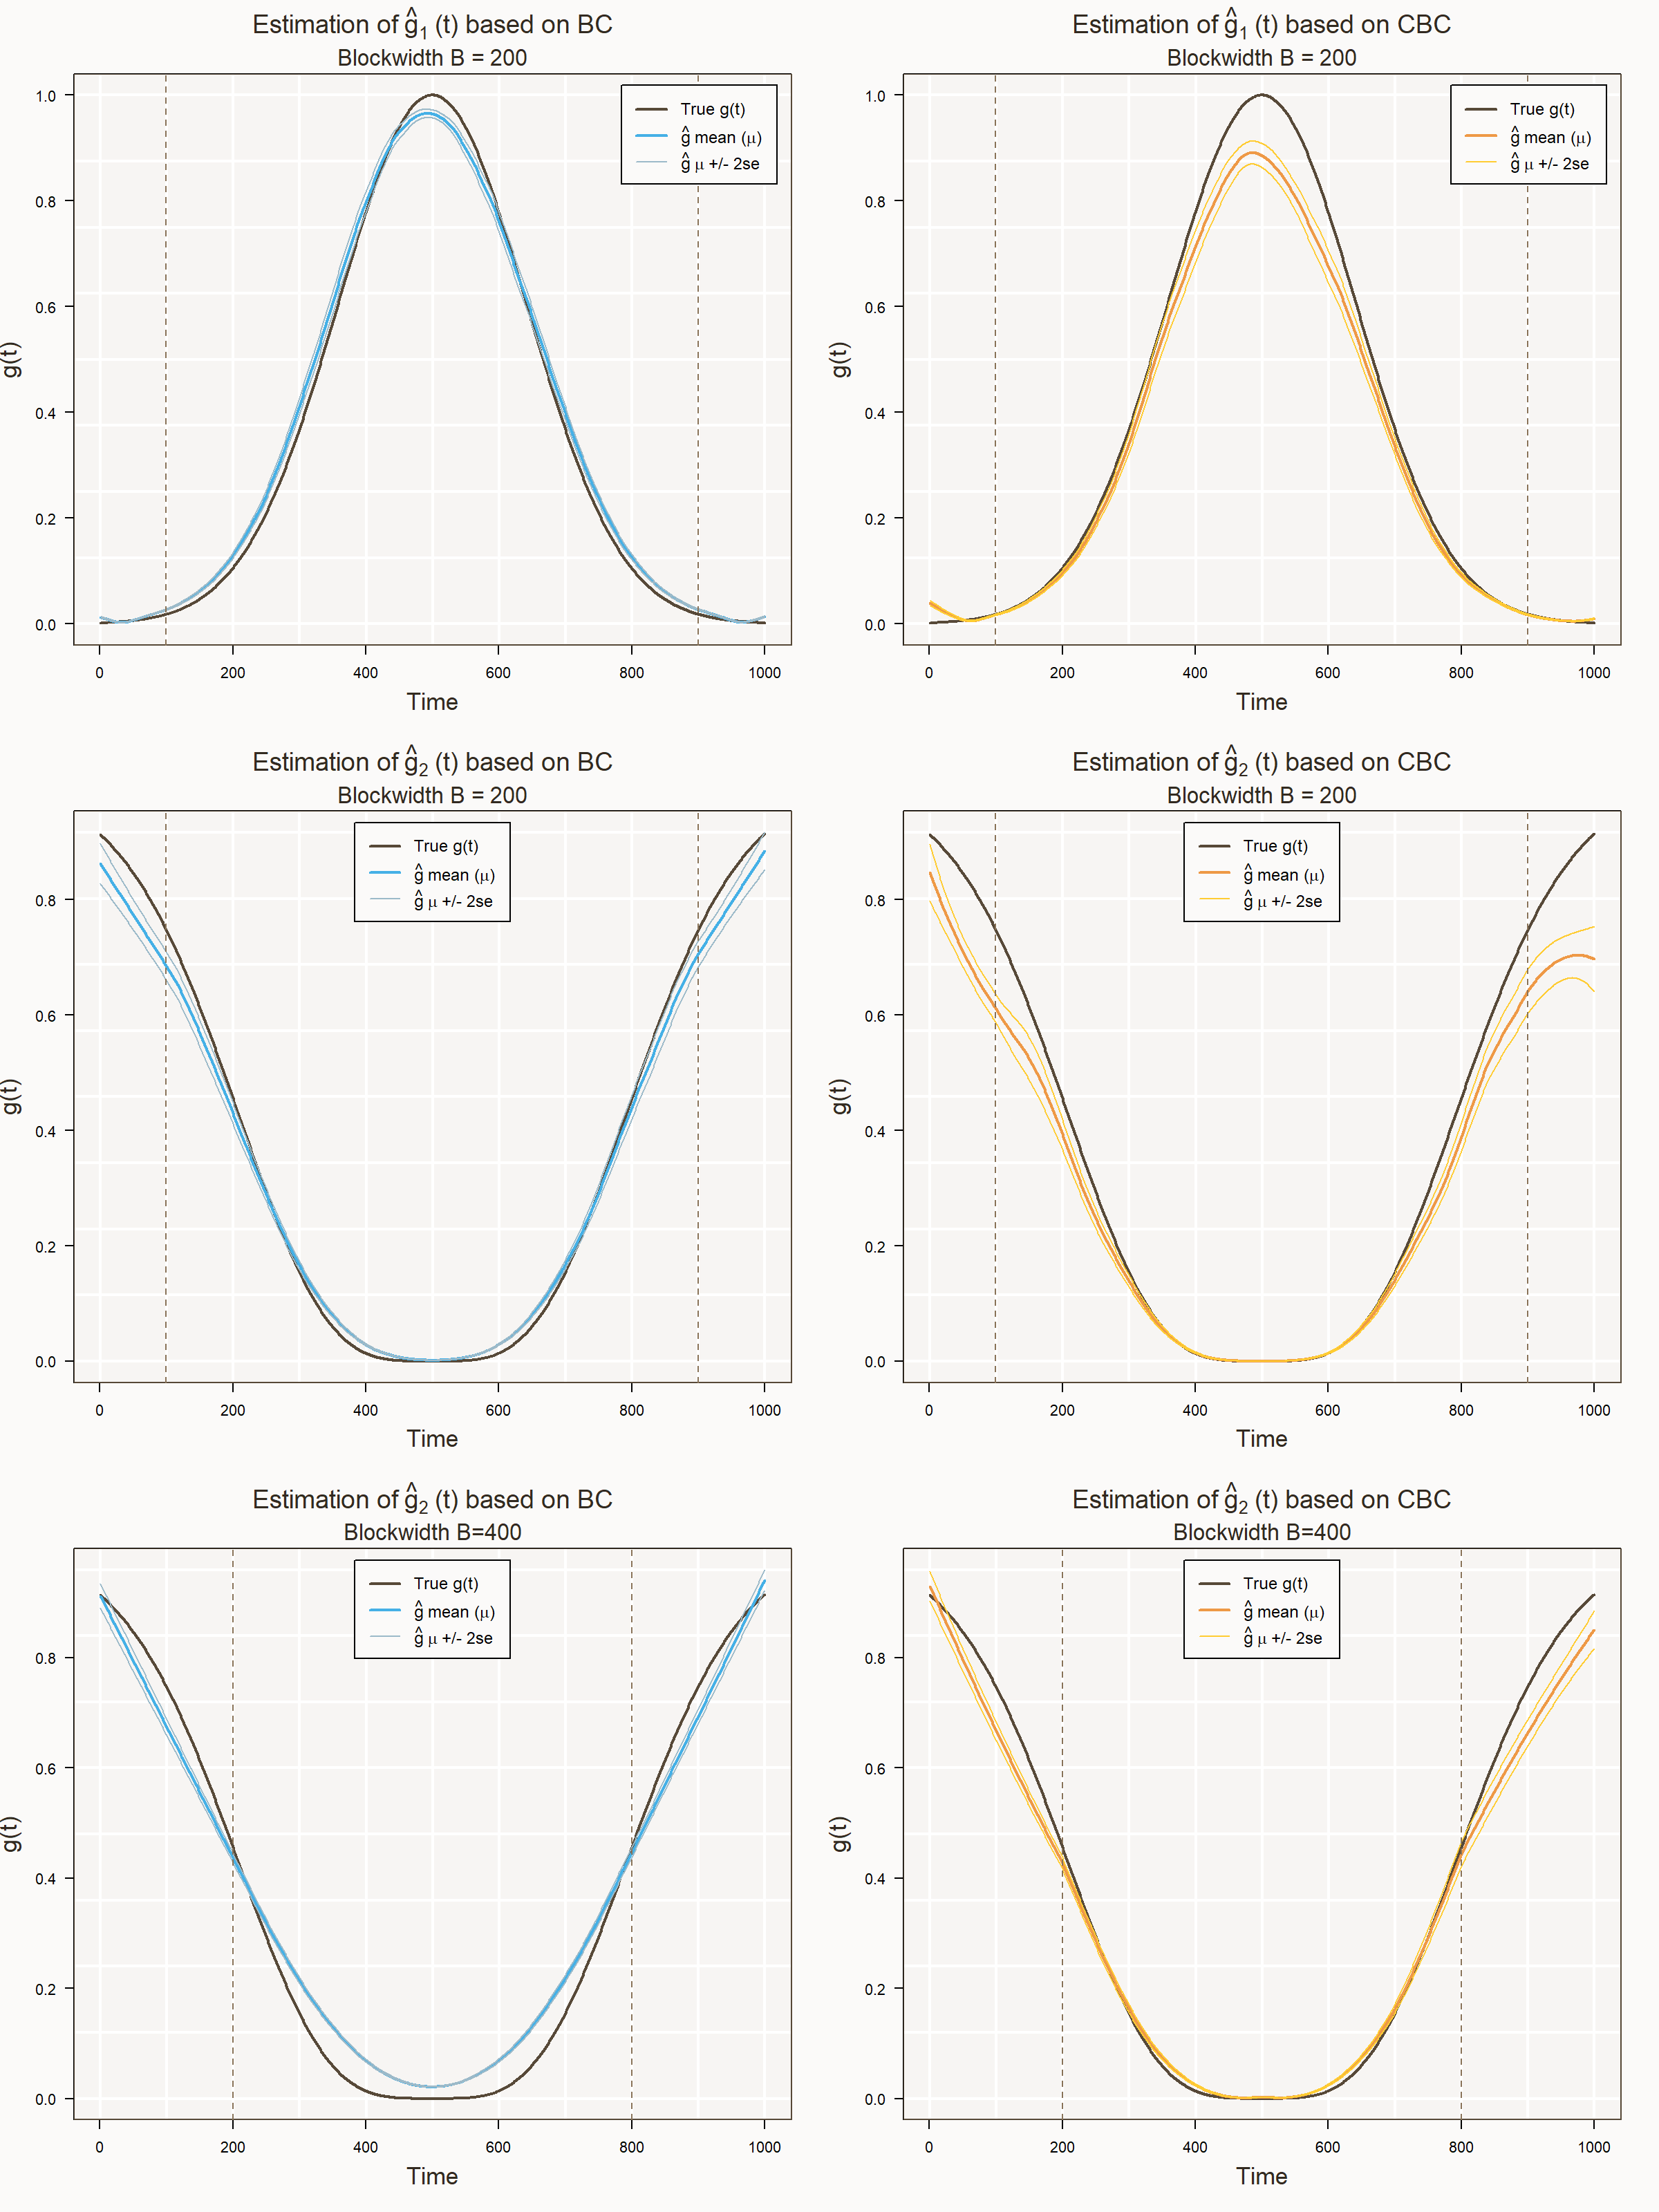
\includegraphics[width=\linewidth]{Fig/gest_UMP_B200_B400.png}
    \caption{}
    \label{fig:enter-label}
\end{figure}


\textbf{Now compare to Azadeh's method if possible}

\section{Using BLABLABLA to Smooth UMP Spectrograms}

As emphasized in the previous section, a convenient and defining attribute of UMPs is that their frequency structure retains constant proportions over time, despite the total power's time-dependency. It makes sense then, that as the outer product of a squared modulating function $g$ and a power spectrum $S_Y$: the TFS of a UMP should give insight into $g$ via it's \textit{rows}, and insight into $S_Y$ via its \textit{columns}.

BLABLABLA more intro stuff

\subsection{Derivation of Techniques}

Consider, again, a UMP $X(t) = c(t)Y(t)$. Let $Q_X$ be the function of frequency obtained from taking the column-wise means of the UMPs TFS matrix, $\mathbb S_X$. That is,
\begin{flalign}
    Q_X(f_i) &= \frac{1}{N}\sum_{t=1}^N S_X(t,f_i)
\end{flalign}
where the $f_i$ are taken from the set of Fourier Frequencies $\{f_1, \dots, f_{N_f}\}$. If $X(t)$ is stationary (in other words, if $g(t) = c^2(t)$ is constant with respect to time), then $Q_X(f)$ should directly reflect the frequency spectrum of $Y(t)$. If $X(t)$ is non-stationary, the proportional structure of $Q_X(f)$ should resemble $S_Y(f)$, however: the two functions will differ by some scale factor dependent on the nature of $g(t)$'s evolution over time.

Similarly to the case of estimating $g(t)$ via row sums of $\mathbb S_X$, it may be possible to normalize $Q_X(f)$ to something more indicative of the true $S_Y(f)$, perhaps by way of an eigenvalue problem resembling that of section (??). It is worth investigating whether such an approach would be effective in the frequency domain context.

With estimates for both $g(t)$ and $S_Y(f)$, we now have the tools to build an entirely new estimate of $\mathbb S_X$,
\begin{flalign}
    \hat {\mathbb S}_X &= \hat g \cdot Q_X(f) 
\end{flalign}
Unlike the BC and CBC, whose sliding windows rupture the spectrogram's constant frequency proportions over time, $\hat{\mathbb S}_X $ will force these proportions to adhere to those of $Q_X(f)$ for across \textit{all} rows of the spectrogram. We'll dub the new estimate the \textit{Smoothed} BC (SBC) or Smoothed CBC (SCBC), depending on the spectrogram from which $\hat g$ and $Q_X$ are obtained.

\subsection{Performance Using Simulated Data}

\begin{figure}
    \centering
    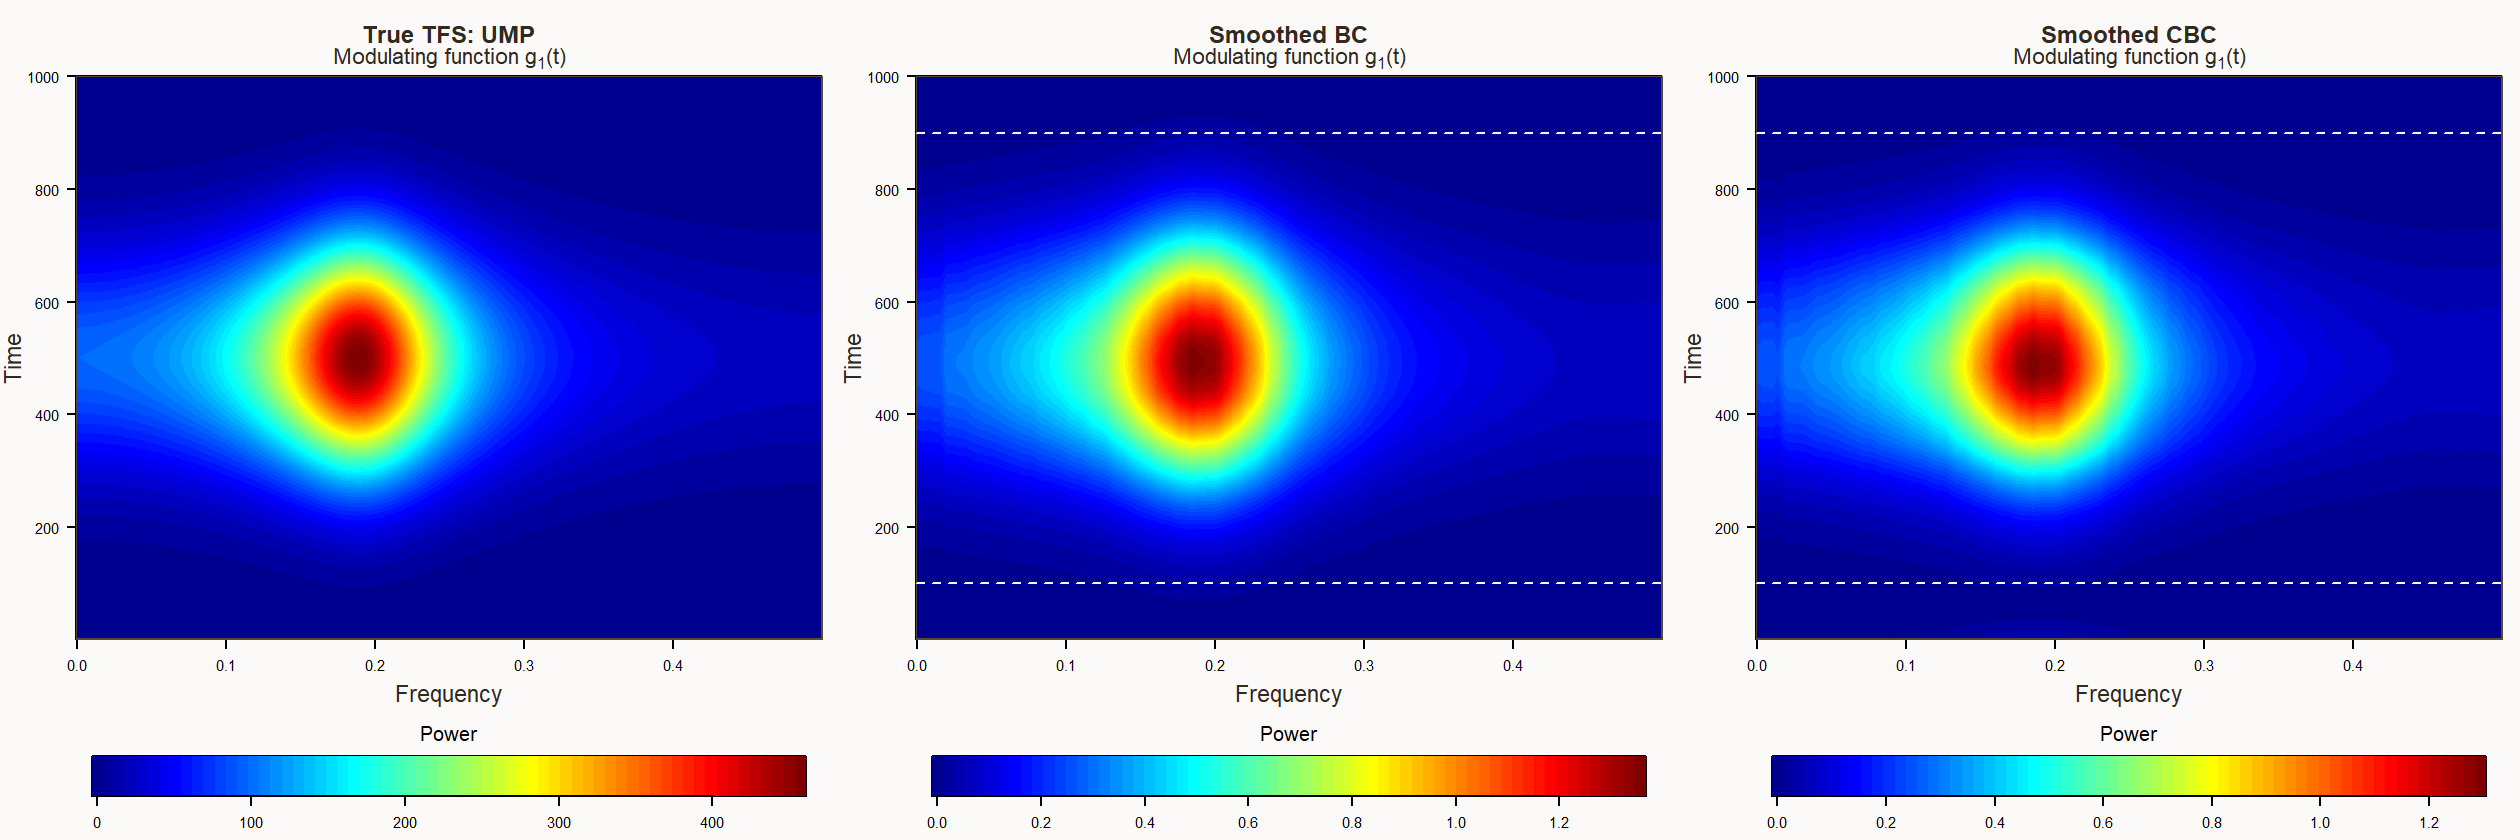
\includegraphics[width=\linewidth]{Fig/smoothgrams_UMP_B200_letterbox.png}
    \caption{M=100}
    \label{fig:enter-label}
\end{figure}

\begin{figure}
    \centering
    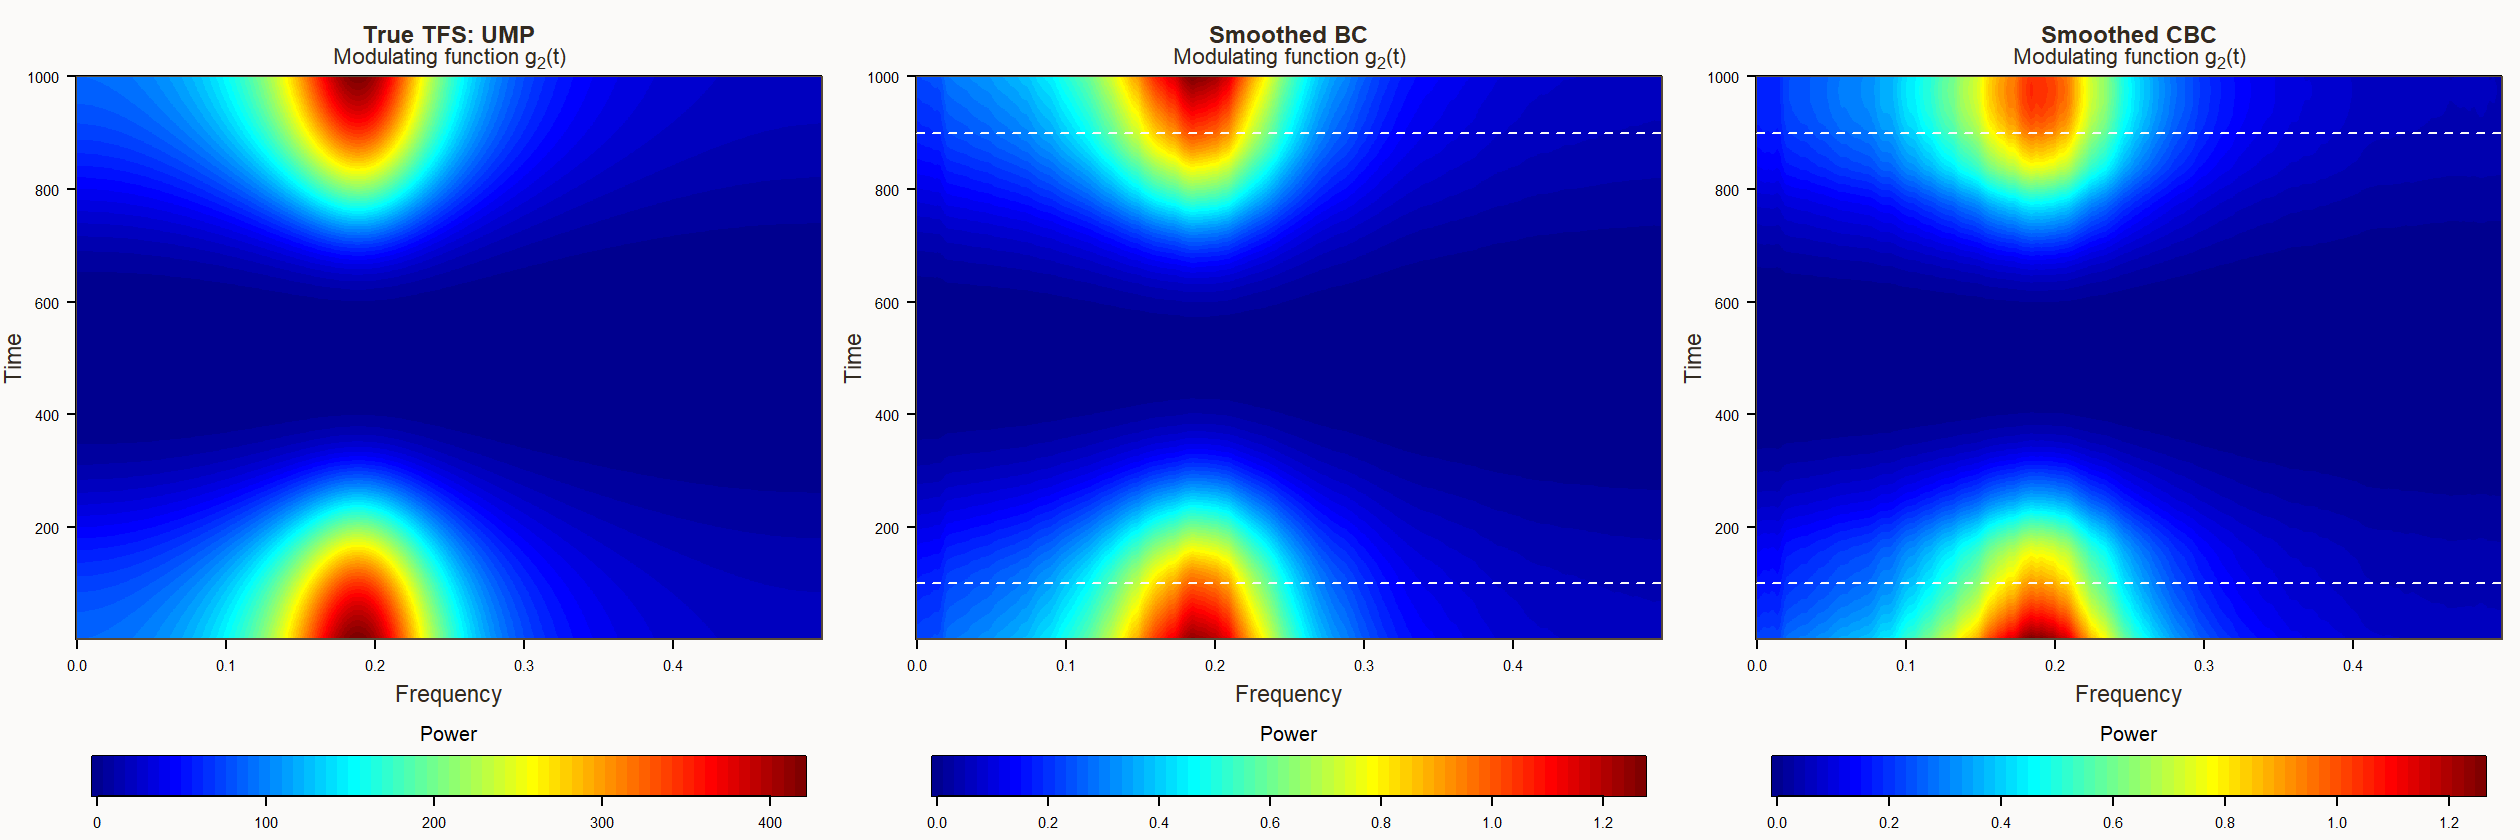
\includegraphics[width=\linewidth]{Fig/smoothgrams_UMP_B200_rev_letterbox.png}
    \caption{M=100}
    \label{fig:enter-label}
\end{figure}

\begin{figure}
    \centering
    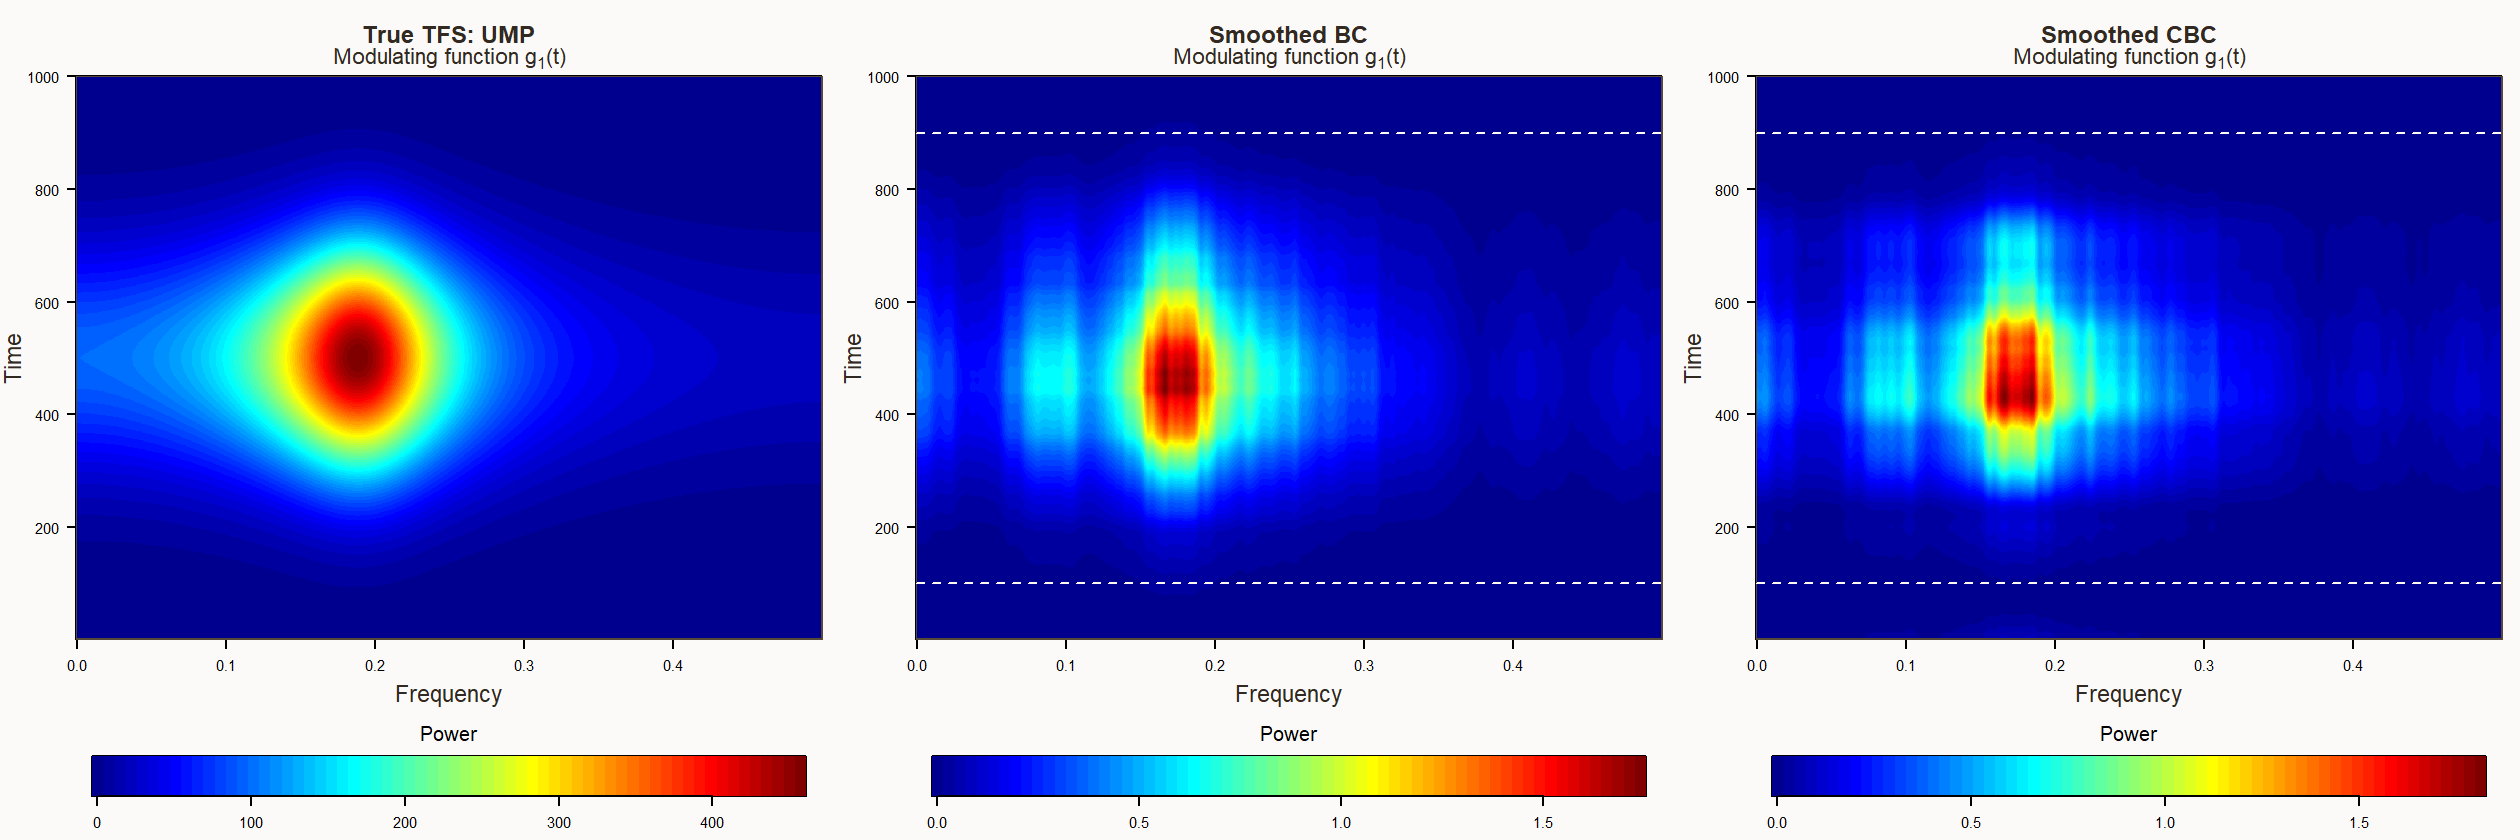
\includegraphics[width=\linewidth]{Fig/smoothgrams_UMP_B200_single.png}
    \caption{M=1 oh my god dude}
    \label{fig:enter-label}
\end{figure}

\begin{figure}
    \centering
    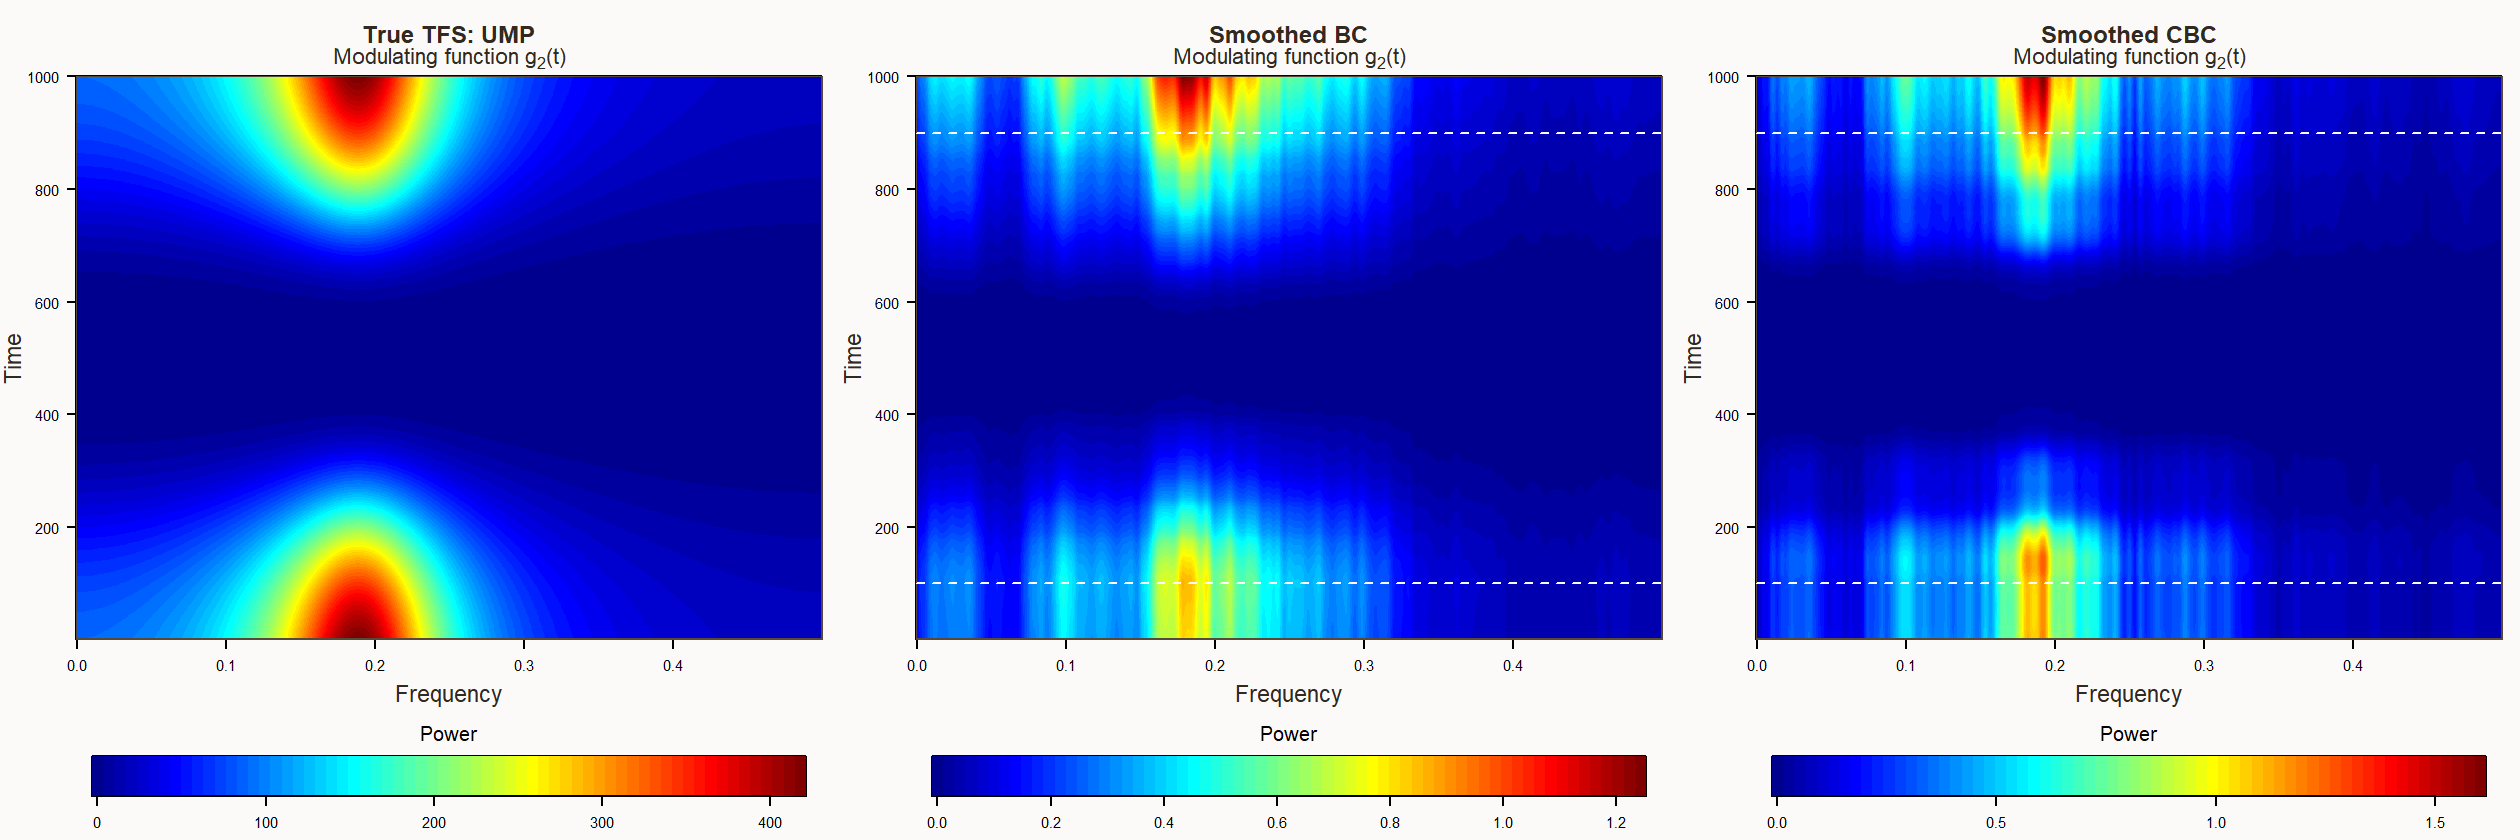
\includegraphics[width=\linewidth]{Fig/smoothgrams_UMP_B200_rev_single.png}
    \caption{M=1}
    \label{fig:enter-label}
\end{figure}

\begin{figure}
    \centering
    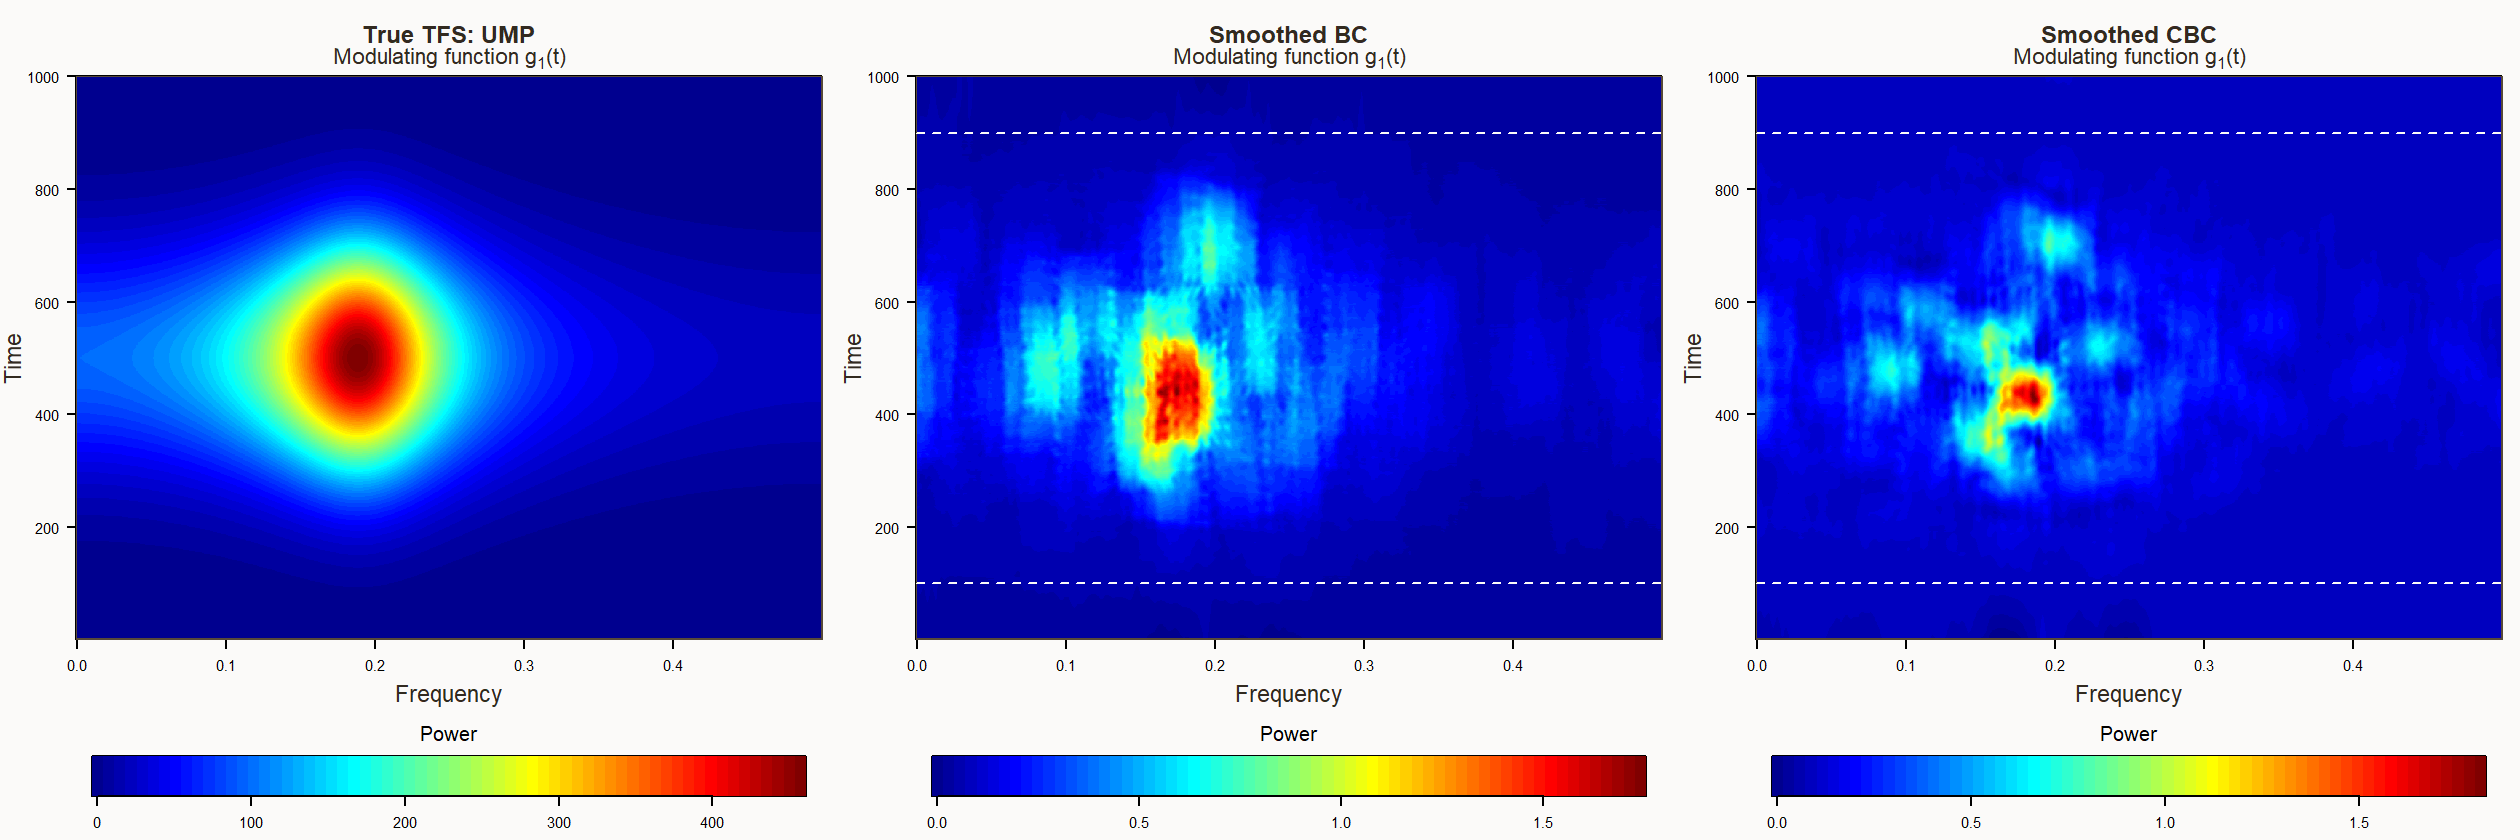
\includegraphics[width=\linewidth]{Fig/smoothgrams_UMP_B200_raw.png}
    \caption{M=1, NO SMOOTH}
    \label{fig:enter-label}
\end{figure}

\begin{figure}
    \centering
    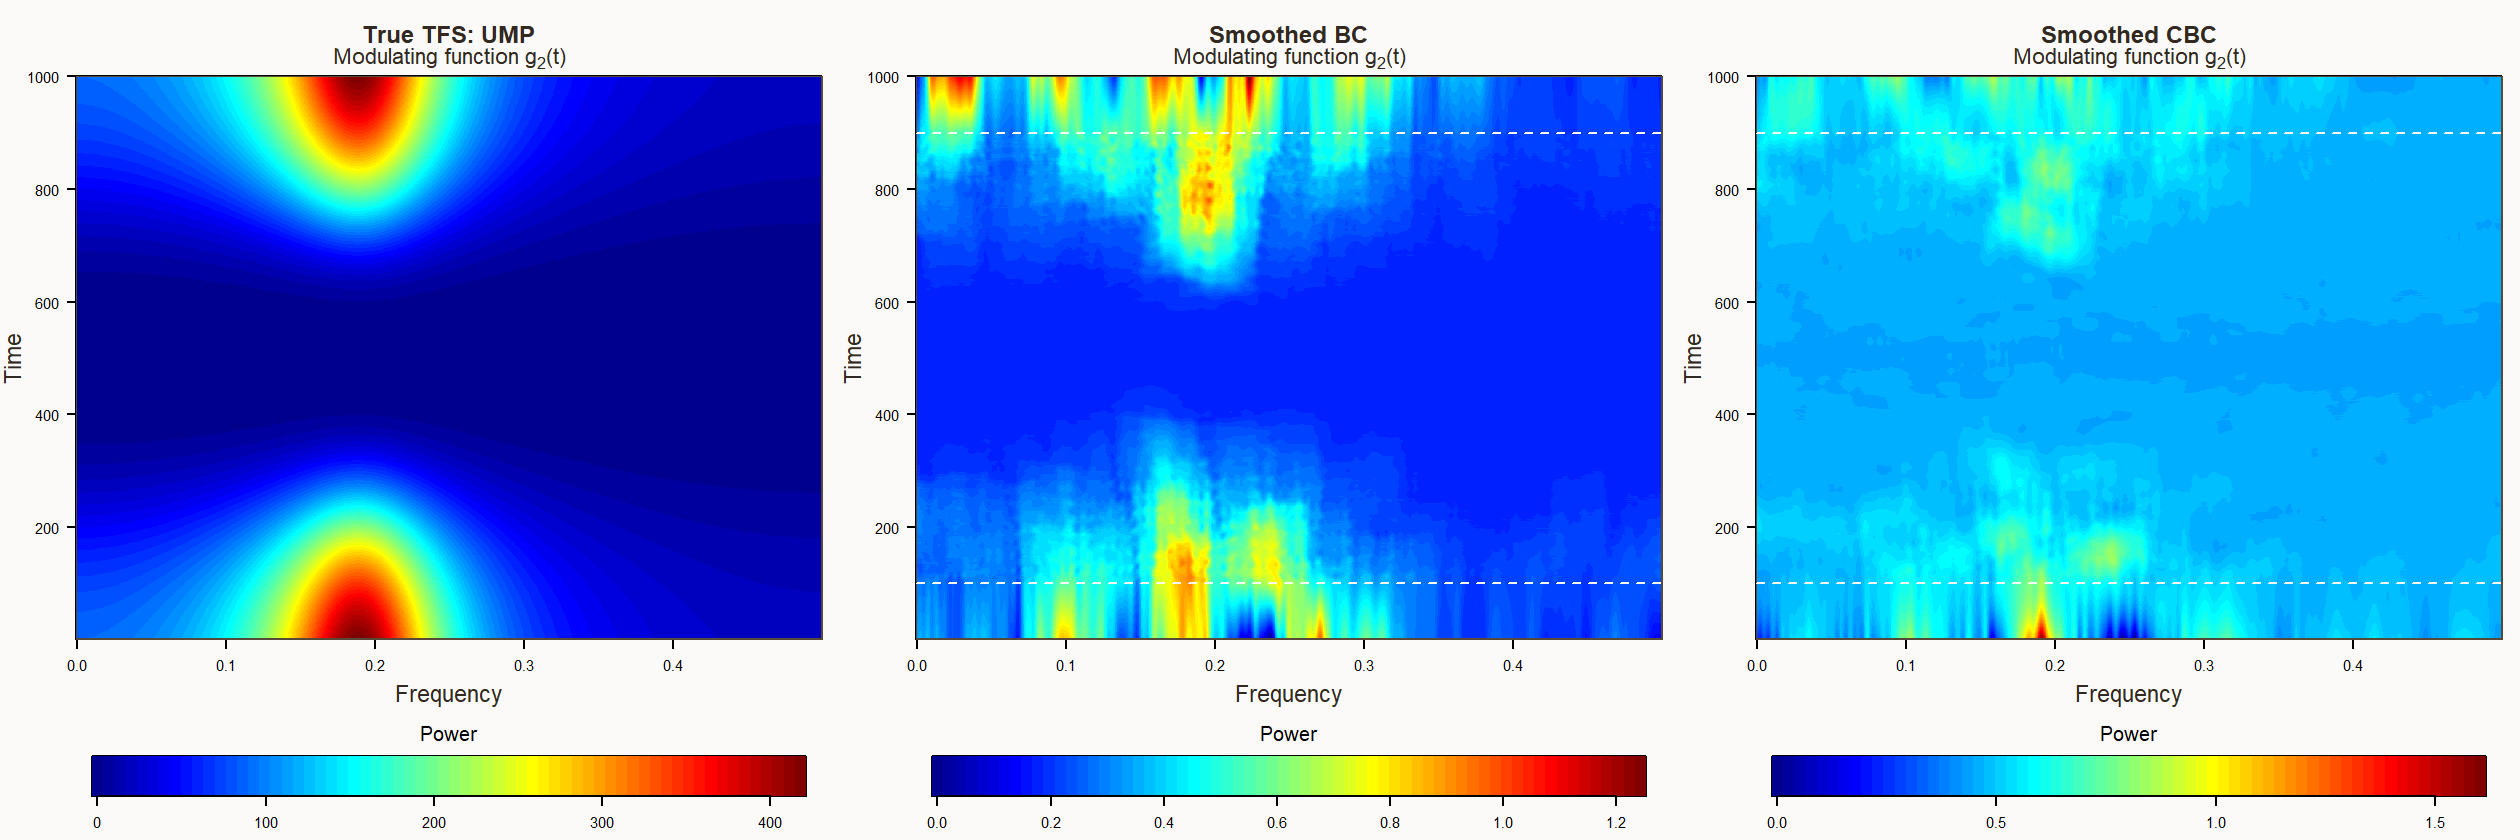
\includegraphics[width=\linewidth]{Fig/smoothgrams_UMP_B200_rev_raw.png}
    \caption{M=1, NO SMOOTH}
    \label{fig:enter-label}
\end{figure}

\end{document}